\chapter{Processing Models}

\section{Motivation}
\begin{definitionbox}{Processing Model}
    A mechanism used to connect operators acting on data in a query.
    \begin{itemize}
        \item Choice is critical to database design.
    \end{itemize}
\end{definitionbox}

\begin{definitionbox}{Function Objects}
    References to code that can be passed, invoked, change state and produce values.
    \begin{minted}{cpp}
#include <functional>

std::function<int(int, int)> add = [ /* captures */ ](int a, int b) { return a + b; }
    \end{minted}
    See \href{https://en.cppreference.com/w/cpp/language/lambda}{C++11 Lambdas}
    \begin{itemize}
        \item Can capture variables (value and references to) (also called closures).
        \item Used to implement single abstract method classes in some languages (e.g kotlin, java)
    \end{itemize}
\end{definitionbox}

\section{Volcano Processing}
\begin{definitionbox}{Volcano Processing Model}
    \begin{center}
        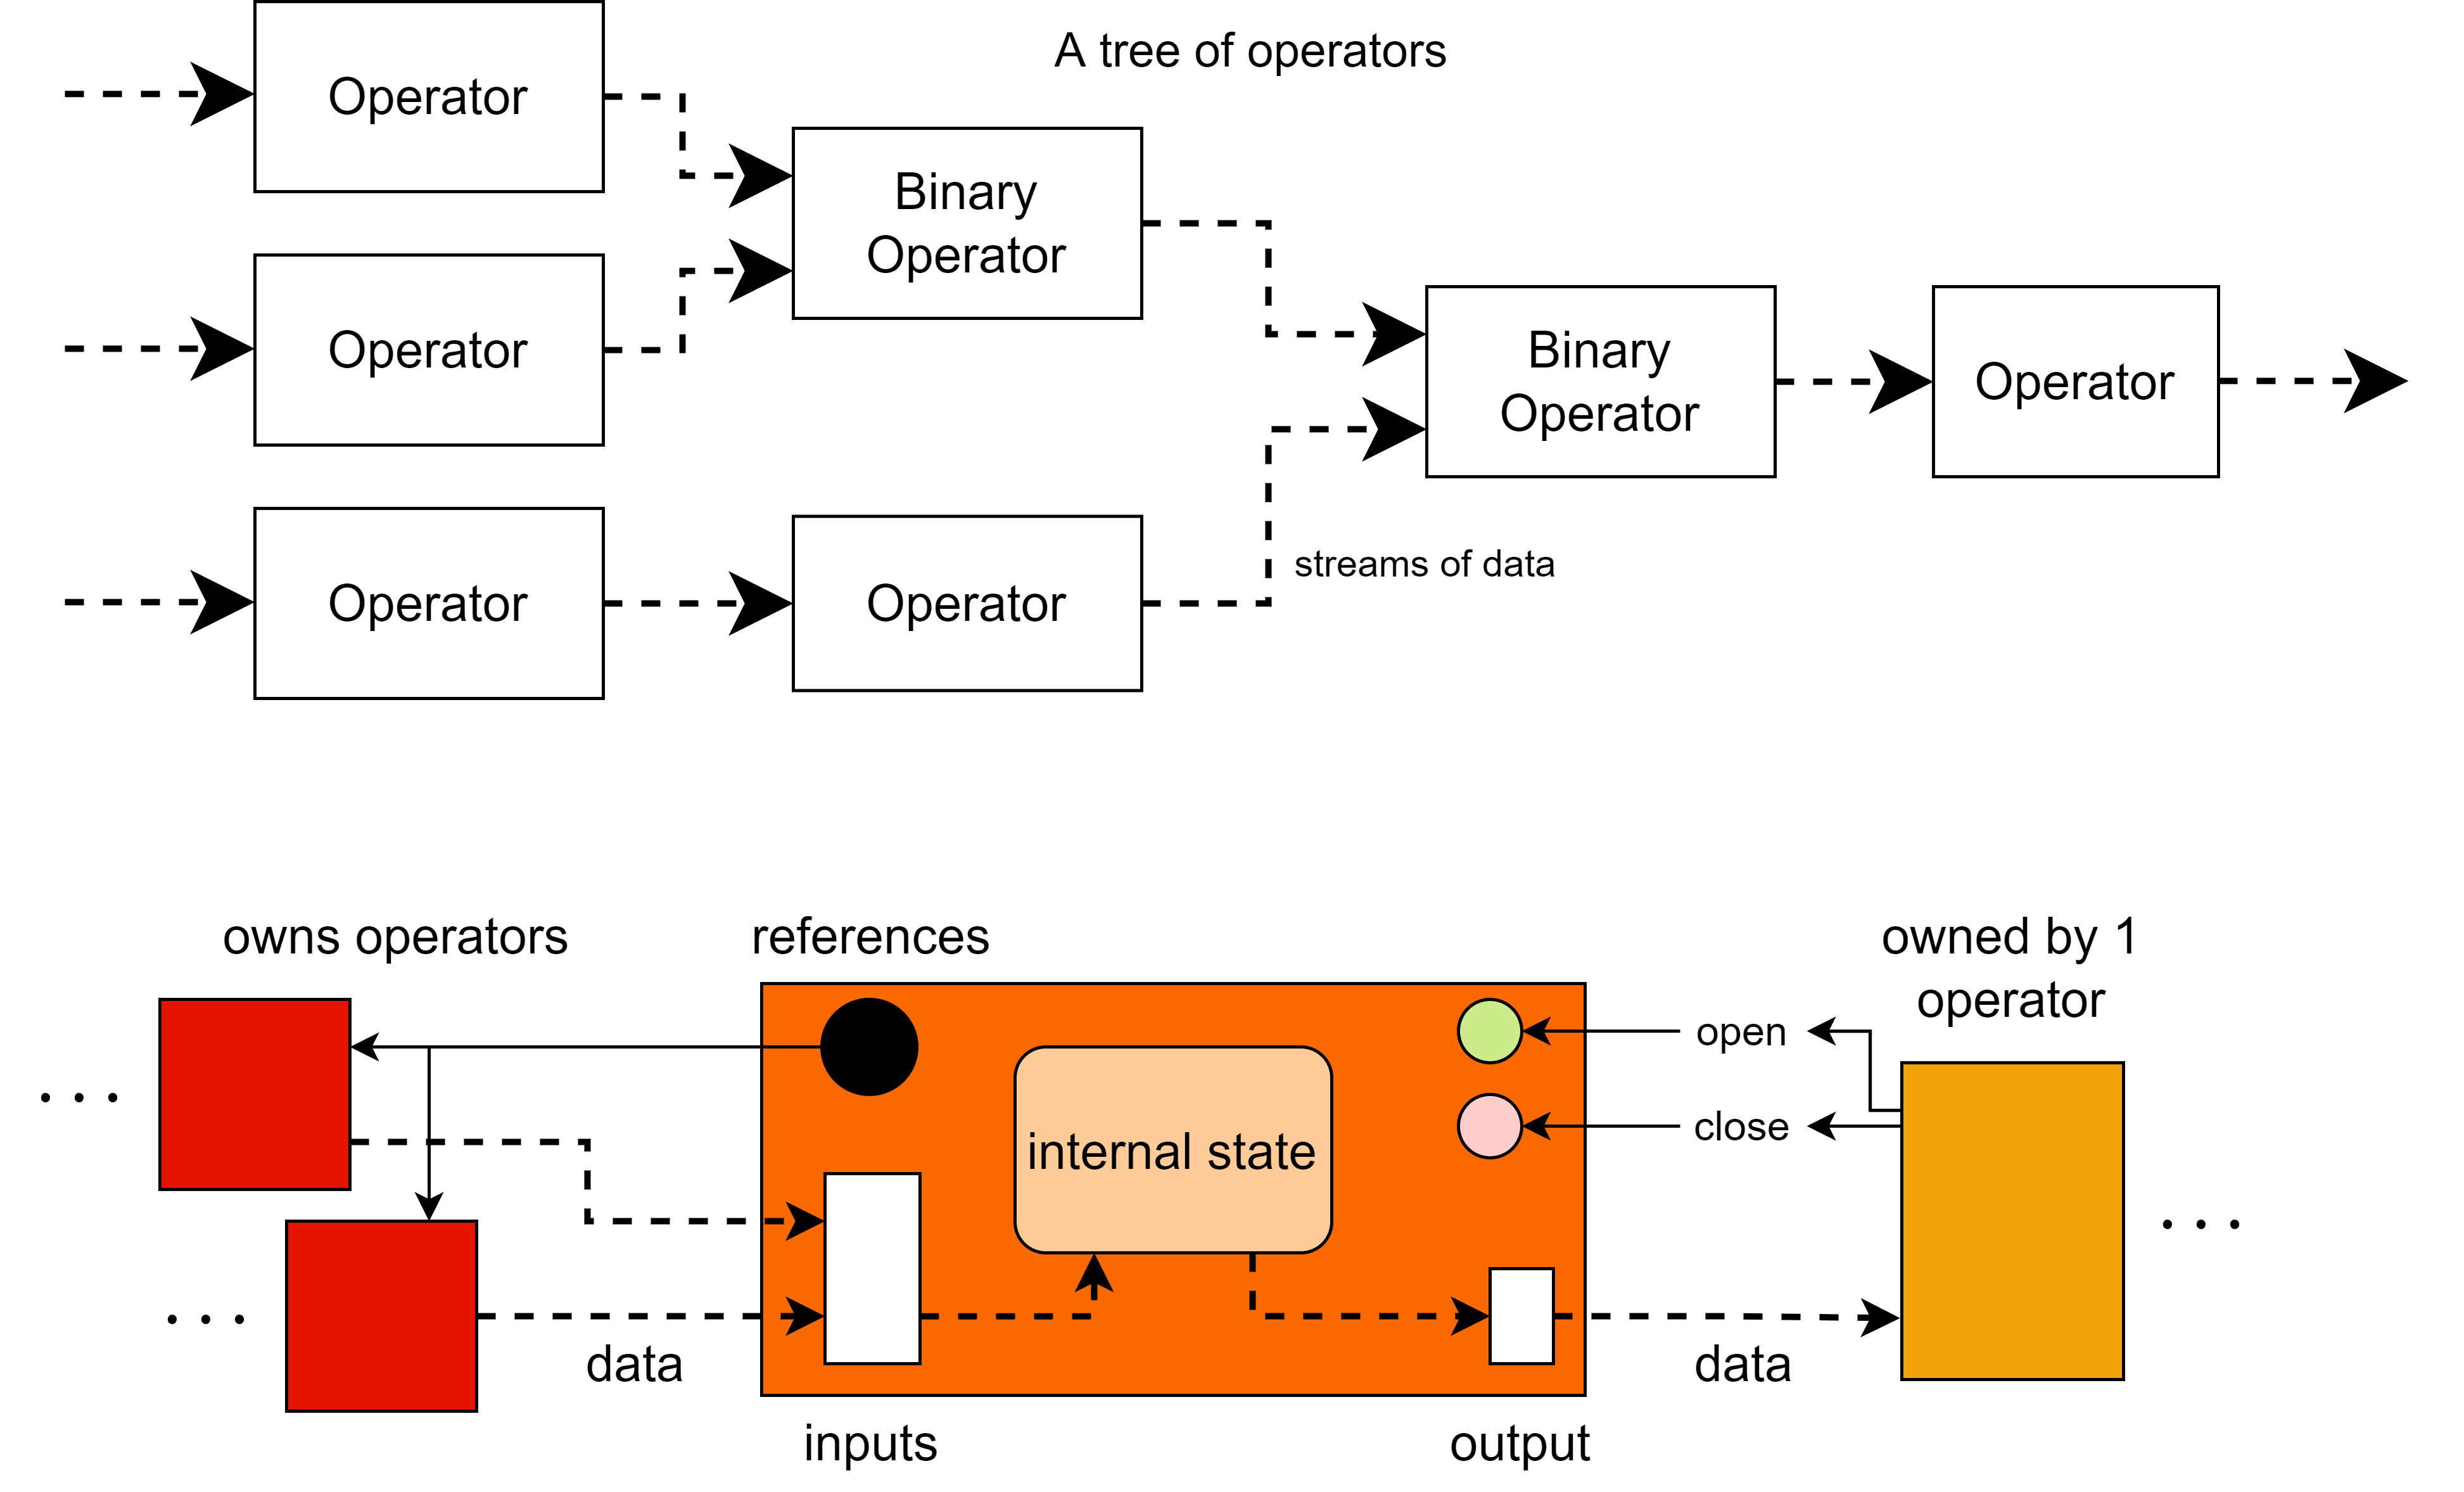
\includegraphics[width=.9\textwidth]{processing_models/images/volcano_stages.drawio.png}
    \end{center}
    Data is fed chunk by chunk (row) through a tree of operators.
    \begin{itemize}
        \item Older design (influential in the 80s) with a focus on design practices over performance. At the time this was an alternative to ad-hoc implementation.
        \item Uses non-relational physical algebra (specialized to be useful in expressing queries for a physical plan, rather than as an abstraction for the programmer).
    \end{itemize}
\end{definitionbox}

\subsection{Operators}
A basic interface for operators can be devised as:
\begin{minted}{cpp}
#include <optional>
#include <tuple>
#include <variant>
#include <tuple>
#include <string>

using namespace std;

/* Variant used -> types for columns only known at runtime */
using Row = tuple<variant<int, double, string>>;

struct Operator {
    virtual void open() = 0;
    virtual void close() = 0;
    virtual optional<Row> next() = 0;
};    
\end{minted}

\begin{sidenotebox}{But why not RAII}
    To keep these examples explicit, an \mintinline{cpp}{open()} and \mintinline{cpp}{close()} are overriden, rather than using the constructor \& destructor.
    \\
    \\ That said RAII would be useful here:
    \begin{itemize}
        \item Automatically clean up after operators after they are dropped.
        \item Cannot be used before open/construction, or used after close/destruction.
    \end{itemize}
\end{sidenotebox}

\subsubsection{Scan}
Scans a table already loaded into memory to return its rows.


\begin{definitionbox}{Pipeline Breaker}
    An operator which can only produce its first value/output tuple after all inputs from one or more input operators has been processed.
    \begin{itemize}
        \item Usually requires some kind of buffering (e.g with \mintinline{cpp}{Difference}).
    \end{itemize}
\end{definitionbox}

